\chapter{Discussion}
\label{chapterlabel7}

\section*{Chapter summary}

In this chapter I will .\newpage


\section{Taxonomy for Media Architectural Interfaces (MAI)}


We would like to relate our findings to the initially examined interaction frameworks, which dealt with the (1) awareness space, (2) actor space, (3) action space and (4) physical space in the context of public displays or a media facade. 
In the following, we will discuss these frameworks in relation to the two design studies as outlined in the last section. 
We argue for the consideration of these multi-layered interaction spaces when designing interactive systems in urban spaces.
\textbf{Awareness space:} In both studies (VEIV London and SCSD Sao Paulo),
the direct interaction activities took place in the immediate vicinity of the TUI, whereas the focal and peripheral awareness spaces differed in their dimensions.
This is firstly due to the dissimilar size of the displays. The display used for the VEIV London study was only 2 by 6 m (i.e. 12 m2) compared to the large media facade for the SCSD Sao Paulo study with 3700 m2.  
At the same time, the difference in distance between the user interface and the display was significant: 5 m VEIV London compared to 33 m SCSD Sao Paulo. 
This seemed to have an impact on people’s spatial awareness with regard to dynamic displays in the city.
\textbf{Actor space:} Compared to the dynamic stream of pedestrians in the SCSD Sao Paulo study, the flow of people in the VEIV London study was rather calm, whilst the event was highly attended. 
The audience hardly changed during the party, but their actions altered; for instance, spectators turned into actors when walking up to the TUI to change the colour of the display and returned to their friends. 
Others simply enjoyed the presence of the colourful display or watched other guests interacting with it. 
In contrast, the dwelling time of the audience during the Sao Paulo event was much lower due to the high pass-through frequency of pedestrians on their way to the underground station.
\textbf{Action space:} The flow of people’s actions during the VEIV London event was different to SCSD Sao Paulo. 
Other than Michelis and Müller (2011) stated, the phases through which people had to go before they could actually interact with the MAI were not stringent in the VEIV London set up. 
People did not necessarily cross in the described order from (1) passing by to (2) viewing and reacting to (3) subtle interactions to (4) direct interactions to (5) multiple interactions and to (6) follow-up actions.
Instead, we observed groups gathering on the lawn walking up to the TUI to collectively explore the interactive system. In contrast to this, we identified human behaviour as explained by Michelis and Müller (2011) during the SCSD Sao Paulo study.
\textbf{Physical space:} The spatial layout in the VEIV London case consisted of a pedestrianised rectangular courtyard enclosed by the historical university buildings, compared to the vibrant two-directional avenue in Sao Paulo, which was lined by high-rise office towers.
In the VEIV London set up, there was hardly any \textit{gap space} in between the TUI and the display (i.e. ca. 5 m), compared to the congested main road in Sao Paulo, which divided the tangible interface from the
media facade (i.e. ca. 33 m). 
In addition, the comfort spaces, potential interaction spaces and social interaction spaces varied greatly in both studies. 
The enclosed courtyard and the positioning of the display within it released more of these spaces than the congested pavement in Sao Paulo.



\subsection*{I'm an Interface}

(insert image from Sentiment Architectures)



\subsection*{Collaboration, team and social dynamics}

Generally speaking the collaboration between a small creative practice and a large resourceful and knowledgeable corporate global company should ideally be of mutual benefit towards prototyping our future city. One may argue that young practices bring in fresh ideas into creative processes, which ideally flourish through the secondment by experienced and established companies. However it comes with some challenges both sides need to be aware of in order not to discourage the others. We were constantly appreciating the expertise and wide experience of Arup engineers and the open mindedness of Arup with regards to exploring new directions in design and architecture. Alongside this we had to accept that the corporate space of a global company his highly controlled in the way that communication leaving the bespoke space needs to be signed off by company officials. This can be cumbersome from time to time as young practitioners are constantly in the need of sharing their activities in form of snapshot images or video footage with their digital networks in order to increase their professional exposure.   

From the beginning of this project the core team consisted of three members; an architect, a lighting designer and a product designer. After we won the competition and the scope of work was clear there was the biggest moment of uncertainty in this project. We had promised a huge design vision for which we did not know how to deliver at this point. This entrepreneurial risk seemed to be too high for one of the core members. As a consequence and after intense attempts to keep him on board the product designer, who was responsible for the digital fabrication, left the team. This caused a vacuum that needed to be closed rapidly. After intensive search we were not able to find a full replacement and decided to split the tasks amongst the remaining two project partners in order to distribute the risks of another failure. Having learnt from this we found it extremely hard to bring a team together that would stick together no matter what challenges may suddenly appear. We found it easy to get people enthusiastic about our project and of course to work with Arup, but finding people with the right skills and commitment was almost impossible within the given time and budget. We learnt that we needed to come up with intangible incentives such as individual creative freedom, access to a professional network and social amenities to convince enthusiasts to come on board. At the same time besides the efforts to find the right kind of collaborators, the core team constantly had to keep the initial design intent in mind to avoid the leaching out through too many concessions towards individual creative freedom. 

\begin{figure}[!h] 
\centering
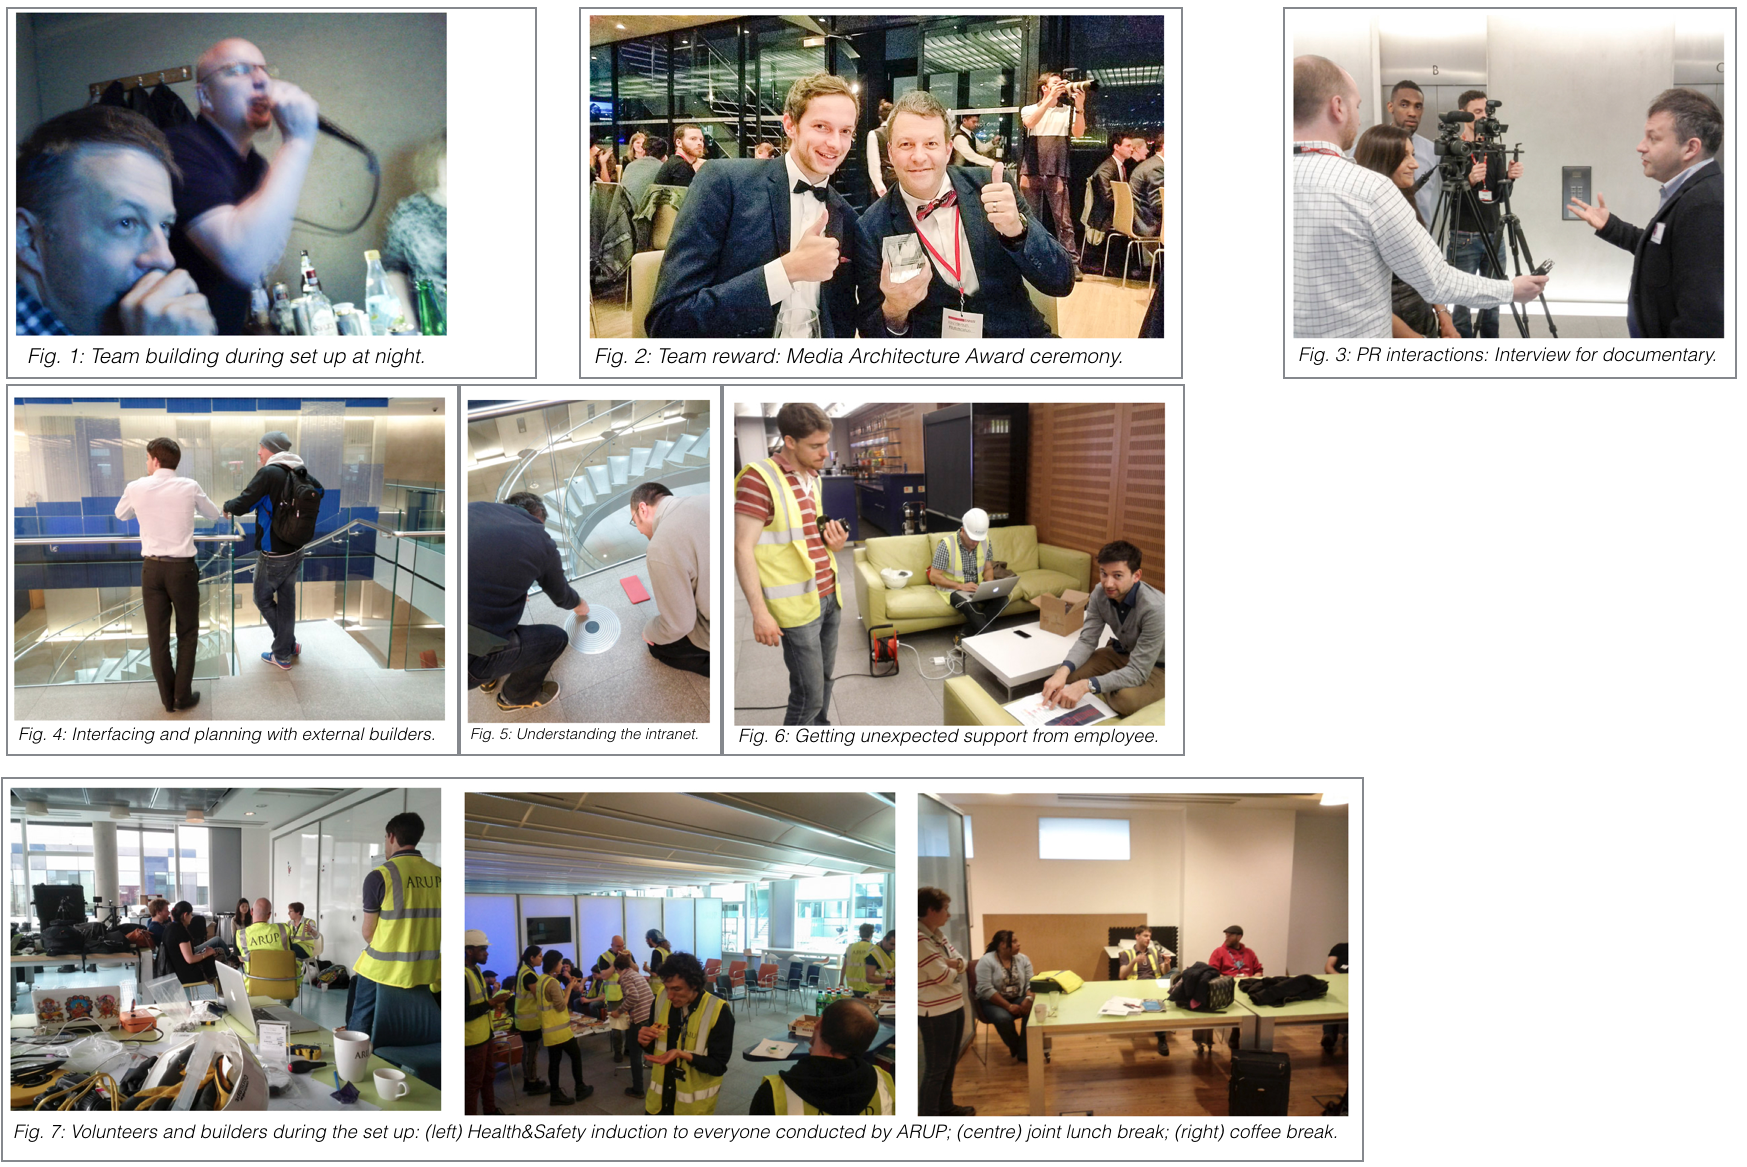
\includegraphics[width=\textwidth]{Illustrations/OnCollaboration.png}
\caption [On collaboration] {On collaboration}
\label{OnCollaboration}
\end{figure}



\subsection*{Managing expectations – the client relationship}

As a matter of fact the different parties involved in this project wanted to achieve the same goals (i.e. completion of the Sentiment Cocoon) their motivations however were different. For Arup it seemed to be the priority to showcase the Cocoon as a structure as well as a vision for better workplaces to their clients in order to demonstrate Arup’s ability to innovation and to support new designers through this competition.
For us as the designers and researchers it was preliminary important to materialise and implement our vision and the containing research knowledge. And of course to increase our professional network, by showing our skills. 
At the same time, managing expectations was a tricky venture throughout the project. For instance when initially proposing a 3D printer during the competition people actually expected what they considered a 3D printer. When we came up with a pallet-wrapping robot, they were rather disappointed of this creature that looked more like a vacuum cleaner. However, considering the fact that the robot quickly got a name (i.e. Einstein) seemed to be a sign of some kind of affection. In addition, calling the new surface a cling film structure made the whole process of wrapping Cocoon sounded a bit trivial. 
Another issue rose when we were calling the pallet-wrapping machine a robot. The health and safety department was particularly concerned about workplace safety. An autonomous machine in an office space would have been an uncontrollably risk. Only when we demonstrated that this machine is not acting like an industrial robot arm being able to cause severe damage we were able to convince the person in charge to sign off this fabrication process.
In a nutshell, the challenge for a successful client relationship is a careful management of expectations.

\section{Social implications}



\subsection{Mediated behaviours}

\subsection{Longitudinal Aspects and Sustainable Interactions}



From a long-term perspective, the rate of direct interactions with the cocoon dropped considerably after five weeks. 
A reason for this could be that many users now seemed to understand how the cocoon worked and might have become tired of it. 
The data sets suggest that this started after week five of the deployment.
In the following weeks, peaks could be identified at certain events, such as the Arup summer party on Tuesday, July 14th. 
In particular, the transition from the novelty effect to the levelling off phase is a highly relevant observation that needs further exploration.



\begin{figure}[!h] 
\centering
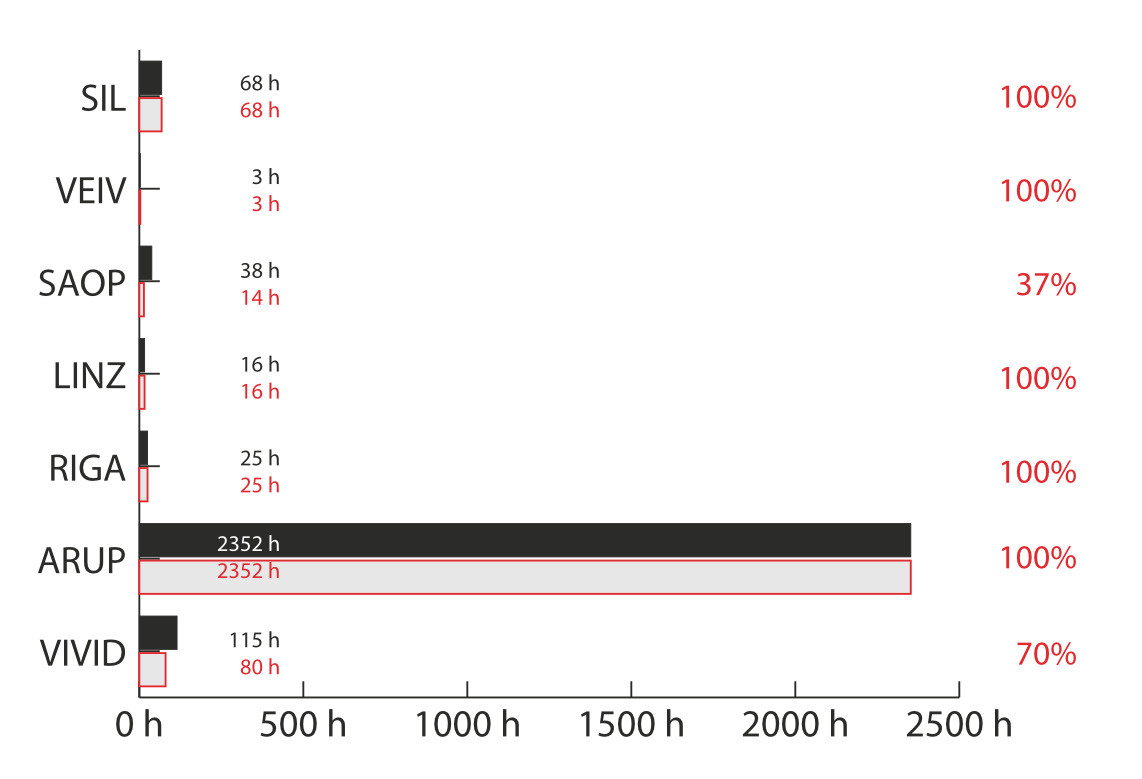
\includegraphics[width=\textwidth]{Illustrations/OverallStudyTimes.png}
\caption [Overall study times] {Overall study times.}
\label{OverallStudyTimes}
\end{figure}



\begin{figure}[!h] 
\centering
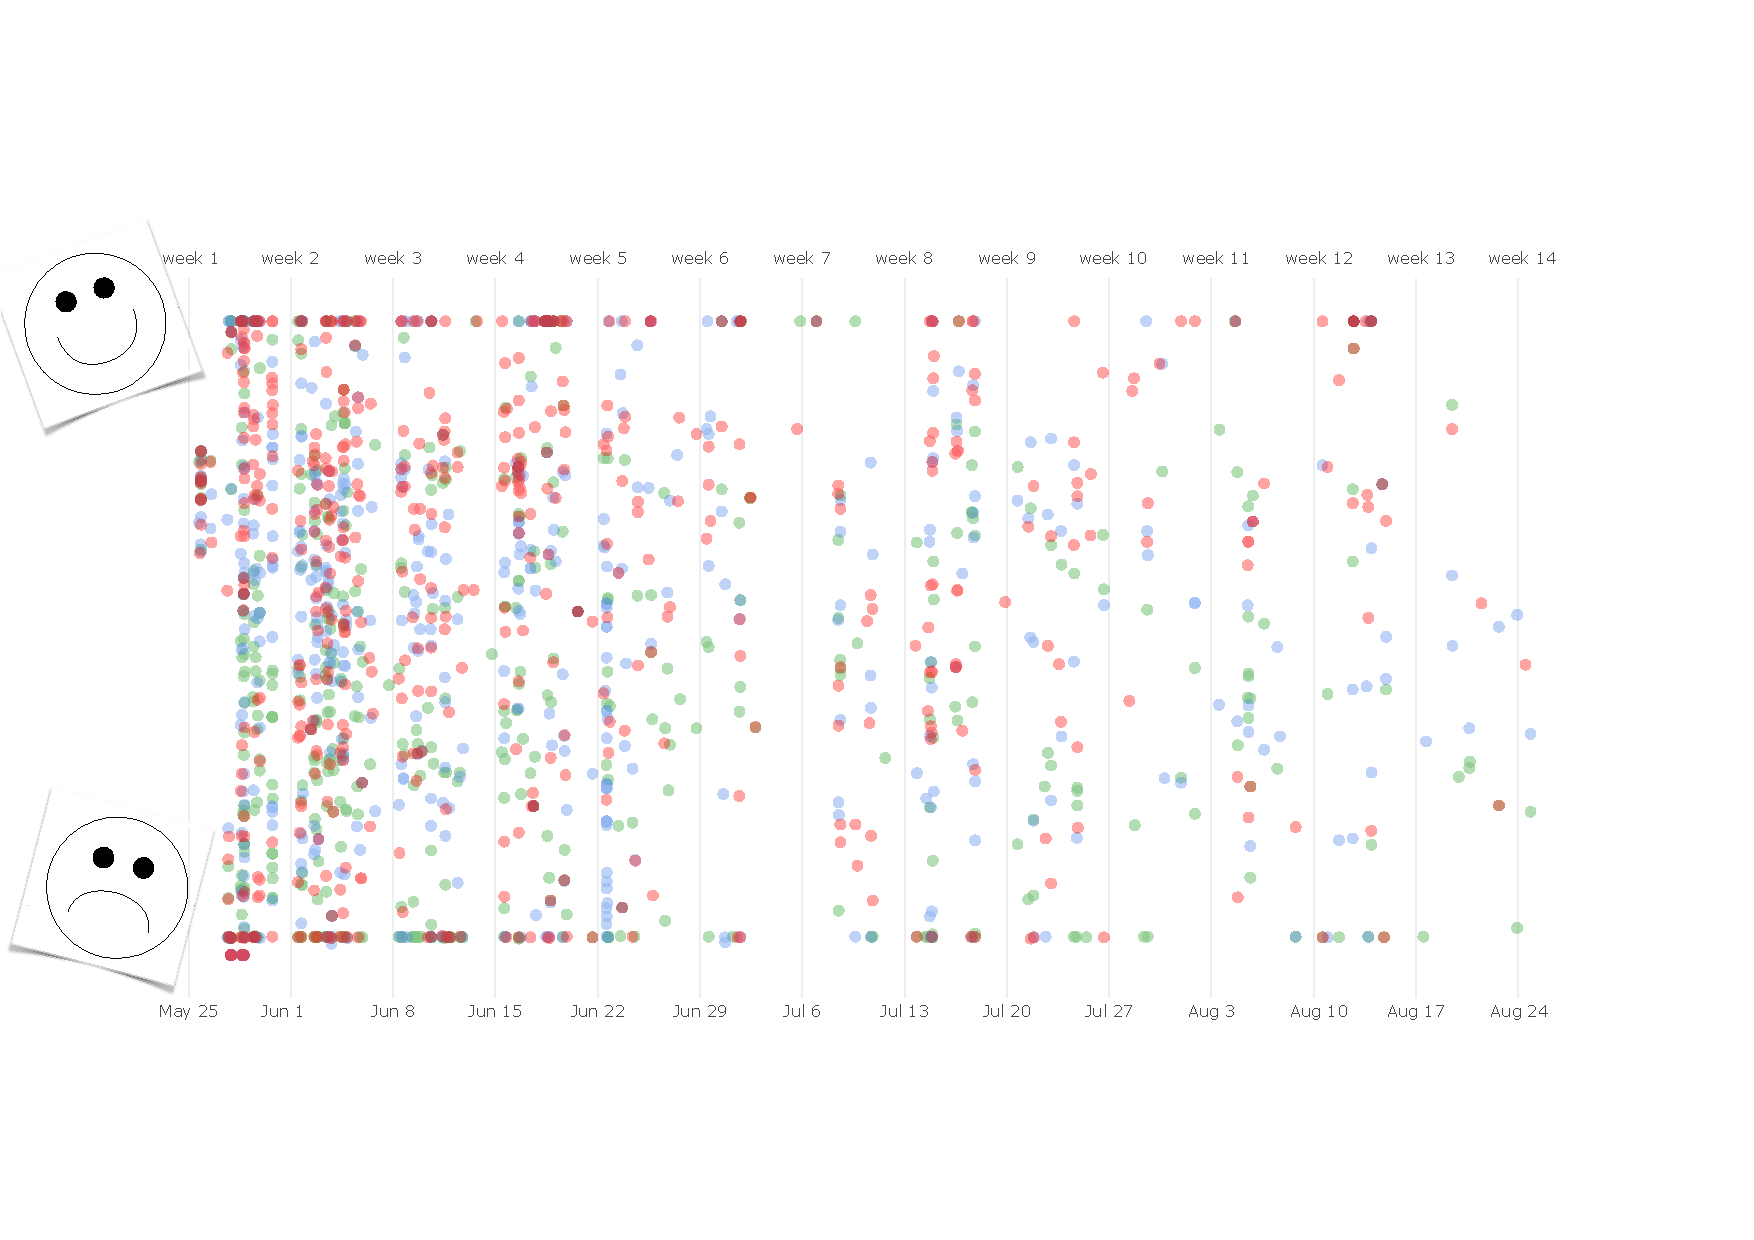
\includegraphics[width=\textwidth]{Illustrations/Sentiment-Analysis.pdf}
\caption [Longitudinal aspects] {Longitudinal data collected during the ARUP study: After week five one can clearly see that interactions with the sentiment interfaces slump.	}
\label{ARUPanalysis}
\end{figure}

\section{Spatial implications}

\subsection{Importance of space}

\subsection{Media architectural scale}

anthropometric scale versus people scale

\subsection{Ambient aspects of Media Architecture}

\subsection{Day versus Night aspects of Media Architecture}

"Despite this increasing urbanisation, we are not using our cities and towns to their fullest potential. Once shops and offices close for the evening, levels of activity in urban centres drop.
Night-time presents challenges to cities globally, be it for reasons of safety and fear, lack of destination or attraction."
Florence Lam, Arup Fellow Global Lighting Design Leader (Cities-Alive-Rethinking-Shades-of-Night.pdf)
\begin{figure}[!h] 
\centering
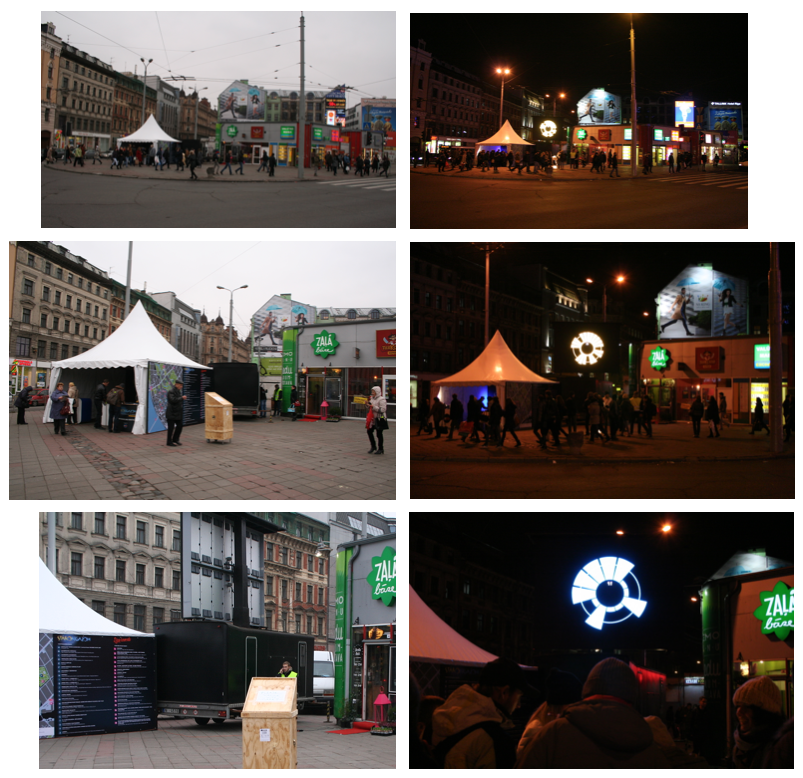
\includegraphics[width=\textwidth]{Illustrations/RIGA_day_night.png}
\caption [Day versus Night aspects of Media Architecture (RIGA)] {During the day the Urban Screen of our media installation was almost invisible within the urban context. During night time the circular appearance of our dynamic visualisation stood out amongst the mostly rectangular displays.}
\label{RIGAdaynight}
\end{figure}


\begin{figure}[!h] 
\centering
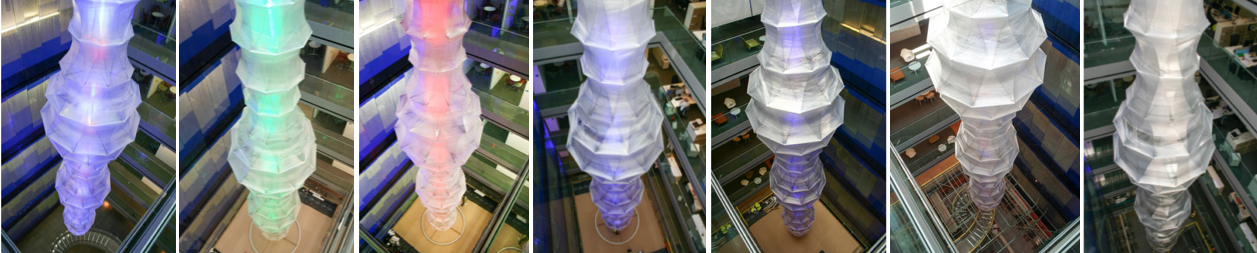
\includegraphics[width=\textwidth]{Illustrations/ARUP_daynight.png}
\caption [Day versus Night aspects of Media Architecture (ARUP)] {Natural daylight, flowing into the atrium from the skylights above, blends with the light emitted by the cocoon’s spine. 
This allows for rich interactions of varying forms of light, which are diffused through the skin of the cocoon. 
The translucency of the material fabricates an effect whereby the suspended cocoon generates a striking visual display of light that has been informed by the feelings of the building’s occupants.}
\label{ARUPdaynight}
\end{figure}

\begin{figure}[!h] 
\centering
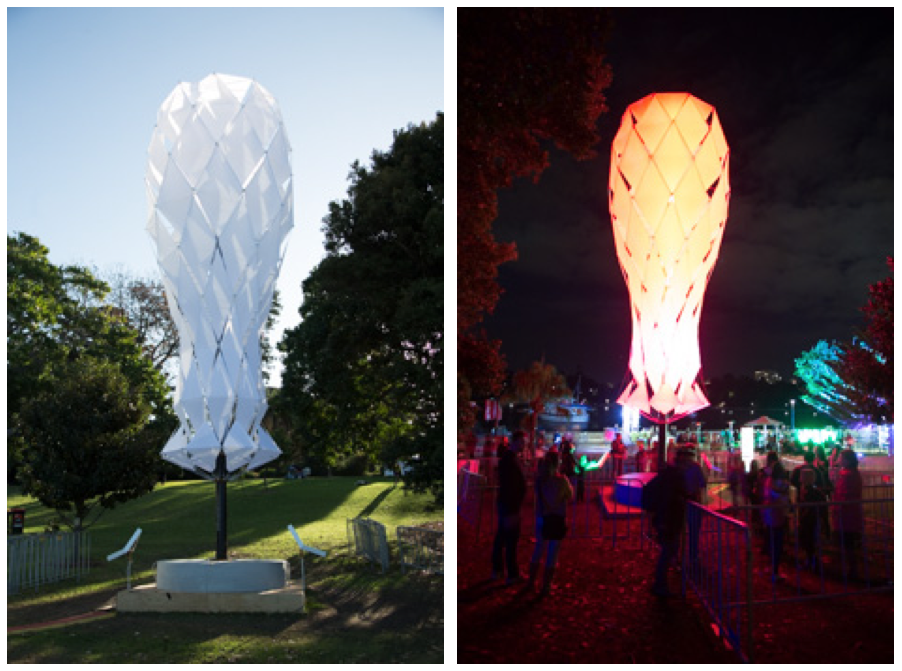
\includegraphics[width=\textwidth]{Illustrations/VIVID_daynight.png}
\caption [Day versus Night aspects of Media Architecture (VIVID)] {Aesthetically pleasing during day and night time: During day the construction and structural pattern of the cocoon become visible, the white sails and the interplay with natural daylight and the sun as well as the wind blowing through the sails creating a constantly changing appearance which develop their own intrinsic quality in contrast to the interactive colourful cocoon during night times. }
\label{RIGAdaynight}
\end{figure}





